% Relevant Safety Standards / Regulations / Markov / ...
% Aircraft System Architectures
% Gamification Concepts / Principles of Game Design
% Review of existing Game Engines / Simulations
% Existing work / state of the art

\chapter{Fundamentals}\label{ch:fundamentals}
In this chapter, the foundations in order to understand the context and to classify this work as a whole will be provided.
The definitions of the most common terms used for aircraft system architecture and the formulas for calculating the relevant
parameters such as failure probability, integrity and safety effect, as well as the foundation of failure analysis are briefly explained in section~\ref{sec:system-architecture}.
Furthermore, as the scope of this work is to implement a game, some basic understanding of games and the game development process, especially in regard
to developing games with an educational approach and idea is described in
section~\ref{sec:game-design}.

\section{System Architecture}\label{sec:system-architecture}
The process of aircraft system design involves multiple stages, starting with requirements gathering.
During this stage, the design team gathers information about the intended use of the aircraft, the desired performance goals, and any relevant safety and environmental regulations.
This information is used to define the design requirements for the aircraft system.
\\
Once the requirements are defined, the design team moves on to the conceptual design stage.
Here, they develop initial design concepts that meet the requirements defined in the first stage.
These concepts may involve trade-offs between different design factors such as weight, cost, and performance.
\\
After the conceptual design stage, the design team moves on to the preliminary design stage.
During this stage, the design concepts are refined and evaluated in greater detail.
The team may use computer simulations and testing to assess the performance of the aircraft system under different conditions.
\\
Once the preliminary design is complete, the detailed design stage begins.
During this stage, the team creates detailed designs for each component of the aircraft system, such as the propulsion system, avionics, and control systems.
These detailed designs must meet the requirements defined in the first stage and be compatible with the other components of the system.
\\
After the detailed design stage, the manufacturing stage begins.
During this stage, the aircraft system components are manufactured and assembled into the final aircraft.
The manufacturing process may involve multiple rounds of testing and quality control to ensure that the aircraft system is safe, reliable, and meets the design requirements.
\\
Finally, the aircraft system is tested and evaluated during the flight test stage.
Flight testing is critical to validating the performance of the aircraft system in real-world conditions and identifying any issues that need to be addressed before the aircraft is certified for operation.
Once the flight testing is complete, the aircraft system is ready for use in commercial or military applications~\cite{lfs1}.

\subsection{Components}\label{subsec:components}
Various elements within an aircraft system serve distinct functions.
Typically, digital aircraft systems comprise sensors, actuators, data transmission buses,
and control and monitoring techniques, which are integrated into avionics that are suitable for aviation use.
\\
\textit{Sensors} are used to measure different parameters such as angle of attack, temperature, pressure or density.
They may output either analogue or discrete signals, meaning a signal can adopt any value on a scale or only a range of defined values,
such as 1 or 0.
Usually, analogue signals are converted to discrete signals before processing, as computers generally may only work with digital
values.
\\
This signal is passed to a \textit{computer} via a data bus, which then processes the signal by applying control laws and other methods to the
input signals from one (simplex) or more (duplex, triplex, \ldots) sensors.
\\
The output signal from a computer may also either be analogue - for example a valve position in percent - or discrete - for
example a state of a valve, closed or open.
The output signal, again has to be possibly converted from a discrete to an analogue value.
This signal is passed to an \textit{actuator} via a data bus, which then executes the given command based on the input signal,
e.g.\ rotating a control surface.


\subsection{Failure Probability}\label{subsec:failure-probability}
The probability of a failure of a system during a specified point in time $t$ is defined as~\cite{lfs2}:
\begin{equation}
    \label{eq:failure-probability}
    P_f(t) \in [0,1]
\end{equation}
Per default, the failure probability of integrated components in system engineering is assumed as $P_f(t) = 1\e-4$~\cite{lfs2}.
\subsection{Reliability}\label{subsec:reliability}
Reliability defines the probability of a correctly acting system at a specified point in time $t$,
therefore it is the inverse of the failure probability~\cite{lfs2}:
\begin{equation}
    \label{eq:reliability}
    P_k(t) = 1 - P_f(t) \in [0,1]
\end{equation}
\subsection{Integrity}\label{subsec:integrity}
The detection probability of an error in a system is defined as integrity~\cite{lfs2}:
\begin{equation}
    \label{eq:integrity}
    C \in [0,1]
\end{equation}
\subsection{Safety Effect}\label{subsec:safety-effect}
There exist different categories of safety effects in the CS-25 for aircraft certification that define the requirements of aircraft systems.
In order to achieve successful certification for an aircraft, each system must adhere to the specified requirements, which are determined by the safety effect category.
Table~\ref{tab:safety-effect} shows the different safety categories.
\begin{table}[!htb]
    \centering
    \begin{tabular}{l|l|l}
        Safety Effect    & Safety Effect short & Accepted Failure Probability \\ \hline
        Catastrophic     & CAT                 & $P_f(1h) <= 1e-9$           \\
        Hazardous        & HAZ                 & $P_f(1h) <= 1e-7$           \\
        Major            & MAJ                 & $P_f(1h) <= 1e-5$           \\
        Minor            & MIN                 & $P_f(1h) <= 1e-3$           \\
        No Safety Effect & NSE                 & $P_f(1h) < 1$
    \end{tabular}
    \caption{Definition of safety effect categories~\cite{lfs1}}
    \label{tab:safety-effect}
\end{table}
\subsection{Common Cause Failure}\label{subsec:common-cause-failure}
Common cause failure (CCF) is a term that describes the failure of multiple components at the same time due to the same cause.
The cause for the failure of one component is not a consequence of a failure of another component, but rather the failure reason is from and
external source, such as a lightning strike~\cite{ccf,cmf}.

\subsection{Common Mode Failure}\label{subsec:common-mode-failure}
Compared to common cause failures, common mode failures (CMF) are failures, where multiple components fail equally, where the reason
for failure may be different for each component.
Common mode failures occur due to design defects, maintenance or installation errors and errors during the development process
of the system~\cite{lfs2,cmf}.

\subsection{Redundancy Concepts}\label{subsec:redundancy-concepts}
As defined in section~\ref{eq:failure-probability}, the default value of integrated aircraft system components is assumed as
$1\e-4$, which means, that with only a single component safety effect requirements of categories higher than \textit{Major} are out of scope.
Therefore, different redundancy concepts have been developed and are being used in system architectures.
These include duplex, triplex and quadruplex systems - meaning, a component is replicated multiple times to run the same program.
One needs to divide between replicated computers, also called \textbf{channels}, and replicated components (e.g.\ CPU) within a computer,
namely \textbf{lanes}.
It is important to note, that each lane or channel is merged right before an actuator and signals in general always join together
at sensors and actuators.
\\
The decision on how the actuator needs to move is done by a \textbf{voting} component, which can have different methods of voting
for the correct output to unify multiple signals into a singular signal: mean value, median value, democratic decision.
The voting component generally is the bottleneck of aircraft systems and needs to guarantee a low probability of failure
due to being the most critical component in the chain, since all further movement is based on its decision.
\\
Actuators can also have a monitoring component, which ensures the correct movement of itself.
This is called a \textbf{Com-Mon} - Command \& Monitoring - system.
It decreases the failure probability, but increases the integrity, meaning that the system is able to react to a possible failure due
to noticing it more reliably.
\\
A number of different concepts is shown in the figures below, which also serves as a guideline to the level design of the game,
since the presentation and understanding of exactly these concepts is the core of the game.
\\
\begin{figure}
    \begin{center}
        \scalebox{0.33}{
            \begin{tikzpicture}[->, >=', semithick, node distance=7cm, auto]
            \tikzset{rectangle/.append style={draw=black, thick, fill=white}}
            \node    (S)[font=\fontsize{24}{0}\selectfont]  {\TBox[fill=white]{Sensor}};
            \node    (C)[font=\fontsize{24}{0}\selectfont, right of=S]  {\TBox[fill=white]{Computer}};
            \node    (A)[font=\fontsize{24}{0}\selectfont, right of=C]  {\TBox[fill=white]{Actuator}};
            \path
        (S) edge (C)
        (C) edge (A);
            \end{tikzpicture}
        }
    \end{center}
    \caption{Simplex System}
    \label{fig:simplex-example}
\end{figure}
\begin{figure}
    \begin{center}
        \scalebox{0.33}{
            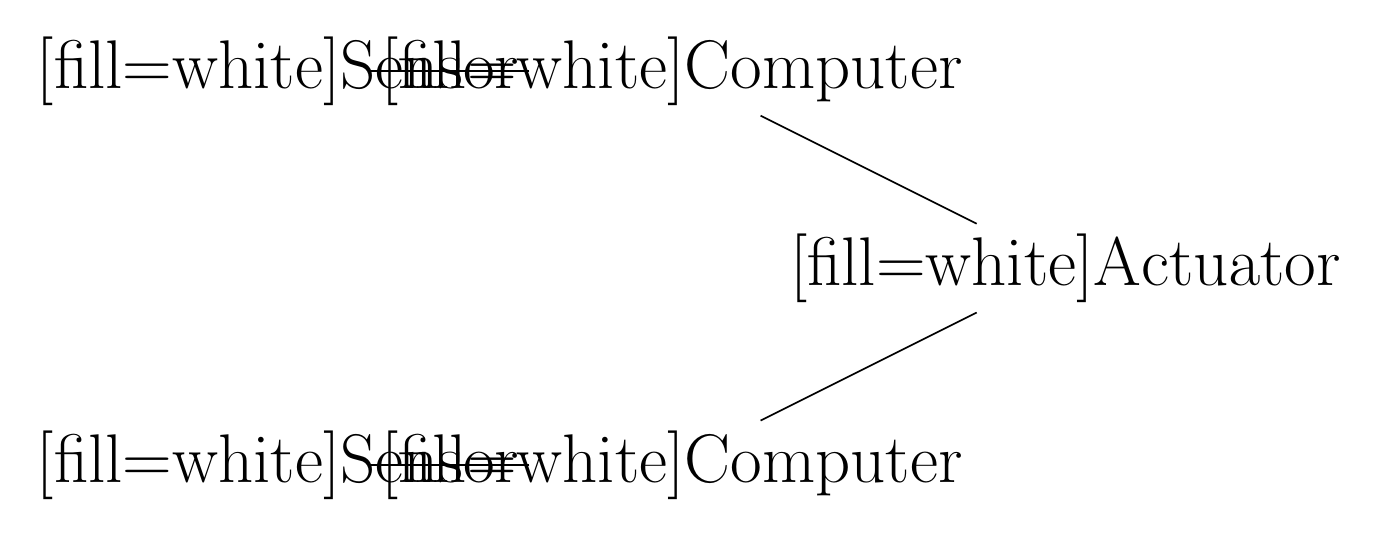
\begin{tikzpicture}[->, >=, semithick, node distance=5cm, auto]
            \tikzset{rectangle/.append style={draw=black, thick, fill=white}}
            \node    (S1)[font=\fontsize{24}{0}\selectfont]  {\TBox[fill=white]{Sensor}};
            \node    (S2)[font=\fontsize{24}{0}\selectfont, below of=S1]  {\TBox[fill=white]{Sensor}};
            \node    (C1)[font=\fontsize{24}{0}\selectfont, right of=S1]  {\TBox[fill=white]{Computer}};
            \node            (C2)[font=\fontsize{24}{0}\selectfont, right of=S2]  {\TBox[fill=white]{Computer}};
            \node    (A)[font=\fontsize{24}{0}\selectfont, right of=C1, yshift=-2.5cm]  {\TBox[fill=white]{Actuator}};
            \path
    (S1) edge (C1)
    (C1) edge (A)
            (S2) edge (C2)
            (C2) edge (A);
            \end{tikzpicture}
        }
    \end{center}
    \caption{Duplex System}
    \label{fig:duplex-example}
\end{figure}
\begin{figure}
    \begin{center}
        \scalebox{0.33}{
            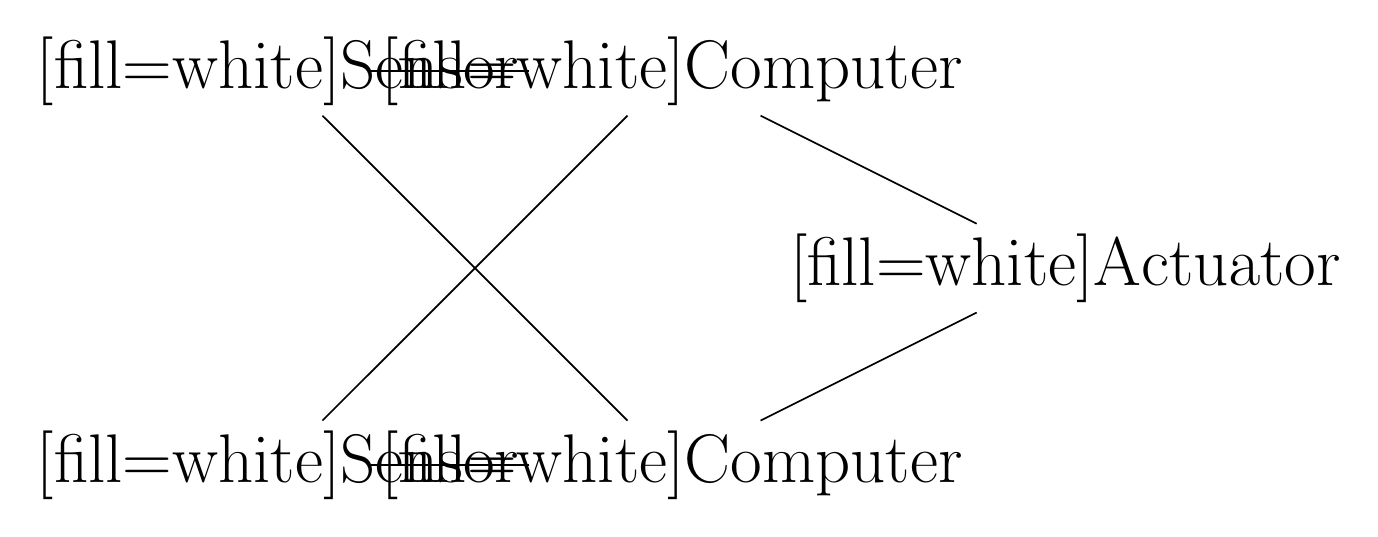
\begin{tikzpicture}[->, >=, semithick, node distance=5cm, auto]
            \tikzset{rectangle/.append style={draw=black, thick, fill=white}}
            \node    (S1)[font=\fontsize{24}{0}\selectfont]  {\TBox[fill=white]{Sensor}};
            \node    (S2)[font=\fontsize{24}{0}\selectfont, below of=S1]  {\TBox[fill=white]{Sensor}};
            \node    (C1)[font=\fontsize{24}{0}\selectfont, right of=S1]  {\TBox[fill=white]{Computer}};
            \node            (C2)[font=\fontsize{24}{0}\selectfont, right of=S2]  {\TBox[fill=white]{Computer}};
            \node    (A)[font=\fontsize{24}{0}\selectfont, right of=C1, yshift=-2.5cm]  {\TBox[fill=white]{Actuator}};
            \path
    (S1) edge (C1)
    (S1) edge (C2)
            (C1) edge (A)
            (S2) edge (C2)
            (S2) edge (C1)
            (C2) edge (A);
            \end{tikzpicture}
        }
    \end{center}
    \caption{Cross-Strapped Duplex System}
    \label{fig:duplex-cross-strapped-example}
\end{figure}

\subsection{Markov Process}\label{subsec:markov-process}
The aircraft design process generally has to comply with the requirements that are stated in regulatory files such as the FAR 25
in order to qualify for the aircraft certification documents.
There are different guidelines for the conduction of the safety assessment process for aircraft systems, which include the
recommendation of quantitative analysis methods such as Fault Tree Analysis, Dependence Diagrams and Markov Analysis.
While the most widely used method today is the Fault Tree Analysis~\cite{7447967}, the Markov Analysis is used for the backend
part of this work, as it provides a good baseline to calculate failure states of aircraft systems in continuous state space due to the memorylessness behavior
and will therefore be explained in detail.
\\
A Markov process, named after the Russian mathematician Andrey Markov, is a stochastic process that possesses the Markov property,
which is the principle of memorylessness.
This means that the future state of the process depends solely on the present state and is independent of its past states.
In simpler terms, a Markov process is a random process where the probability of transitioning to a new state is determined
only by the current state and not by any prior history~\cite{markov-processes}.
\\
Markov processes can be categorized into two main types:
discrete-time Markov chains (DTMC) and continuous-time Markov chains (CTMC).
In a discrete-time Markov chain, the state transitions occur at discrete time steps (e.g., every second or every day),
while in a continuous-time Markov chain, the transitions can happen at any point in continuous time~\cite{markov-processes, VANKAMPEN200773}.
In the scope of this work, a continuous time markov chain model is used.
\\
To define a Markov process, two main components are required:
\begin{enumerate}
    \item State space: The set of all possible states that the process can be in. The state space can be either finite or countably infinite.
    \item Transition probabilities: The probabilities of transitioning from one state to another state. For a discrete-time Markov chain, the transition probabilities are given by a matrix called the transition matrix, with each element representing the probability of moving from one state to another. For a continuous-time Markov chain, the transition probabilities are given by a matrix called the transition rate matrix, with each element representing the rate at which the process transitions from one state to another.
\end{enumerate}
Outside of aircraft system engineering, Markov processes have a wide range of applications in various fields such as economics, finance, biology, linguistics,
and computer science.
They are used for modeling random phenomena where the memoryless property holds,
including stock price movements, DNA sequences, and speech recognition~\cite{markov-usage}.

\subsubsection{State Space}\label{subsubsec:state-space}
The state space for the markov process in aircraft system design is a finite state space, which is determined through the amount of components
a system consists of and the amount of different types of failures.
Failure types may include mechanical failures, electrical failures or software failures, which can each be categorized as either
passive or out-of-control failures, depending on if the failure was detected or not.
As a result, the markov state space consisting of the possible states of the system items, which in the scope of
this work are the four different states: \textit{correct}, \textit{failed}, \textit{passivated}, \textit{out-of-control}.

\subsubsection{Transition Probability}\label{subsubsec:transition-probability}
The transition probability describes the change of one state to another, which in case of aircraft systems is a type of tree
process, as any ``failed'' state may not be recovered to a correct state, as it is assumed the component is in a defect state until
maintenance or re-installation.
Therefore, the resulting graph of transitions is one directional.
A singular state transition from state $A$ to state $B$ is therefore defined as the failure probability~\ref{eq:failure-probability}
of the component that changes its state
from correct to failed.
Going on from the failed state, as seen in figure~\ref{fig:state-change}, there are two possibilities,
a stange change from $B$ to $C$ shows the failure detection ratio, also known as integrity~\ref{eq:integrity}
and a state change from $B$ to $C$ describes the transition to an undetected (out-of-control) failure.
\begin{figure}
    \begin{center}
        \begin{tikzpicture}[->, >=stealth', auto, semithick, node distance=3cm]
        \tikzstyle{every state}=[fill=white,draw=black,thick,text=black,scale=1]
        \node[state]    (A)                     {$A$};
        \node[state]    (B)[below of=A]   {$B$};
        \node[state]    (C)[below left of=B]   {$C$};
        \node[state]    (D)[below right of=B]   {$D$};
        \path
    (A) edge     node{$p_f$}     (B)
    (B) edge                node{$C$}           (C)
        edge                node{$(1-C)$}           (D);
        \end{tikzpicture}
    \end{center}
    \caption{State transitions for a failure in an aircraft system, example}
    \label{fig:state-change}
\end{figure}
\section{Game Design}\label{sec:game-design}
Game design is the conceptional process taking place at the very beginning of game development.
Tasks such as defining a basic game idea and laying out the game mechanics, describing the different components of the game and
reiterating those during the development are part of a game designers' field of exercise~\cite{10.5555/2544002}.

\subsection{Game Definition}\label{subsec:game-definition}
Games can be defined in very different ways, depending on the perspective.
Typically, it is referred to as a ``\[\ldots\] type of play activity, conducted in the context of a pretended reality, in which the participant(s)
try to achieve at least one arbitrary, nontrivial goal by acting in accordance with rules.''~\cite{10.5555/2544002}
\\
\\
The main elements of a game are, according to the definition of Adams: play, pretending, goal and rules.
\\
\\
Engaging in \textbf{play}, which can be an act of self-amusement, occasionally takes on a serious undertone, as seen within the context of this thesis.
In comparison to books or movies, which are presented to the user, games are instead interacted with directly by the user.
The main difference being, that movies and books are static, while a game may change depending on actions of the user.
\\
\\
\textbf{Pretending} reality means creating an immersive experience which does not necessarily be in sync with the real world.
There may be impossible things or actions, which can be done by the player in a game.
Some activities or games may seem like there is no real immersive experience that needs to be pretended, however almost always there are certain
aspects, that do require some sort of pretending.
A flight simulator serves as an example of this concept, as it is technically considered a game but involves a highly physical activity that can also be performed in reality.
However, someone may not have the possibilities to fly an aircraft themselves or travel the world so simply, which is where pretending comes into play.
The player is pretending to be a pilot. \todo{does that make sense? find better example maybe}
The pretending aspect of games is often referred to as the ``Magic Circle'', as seen in figure~\ref{fig:magic-circle}, where the magic circle represents sort of a
playground that is agreed on by all players which is outside the real world and may be defined by imaginary objects or rules.
\begin{figure}
    \centering
    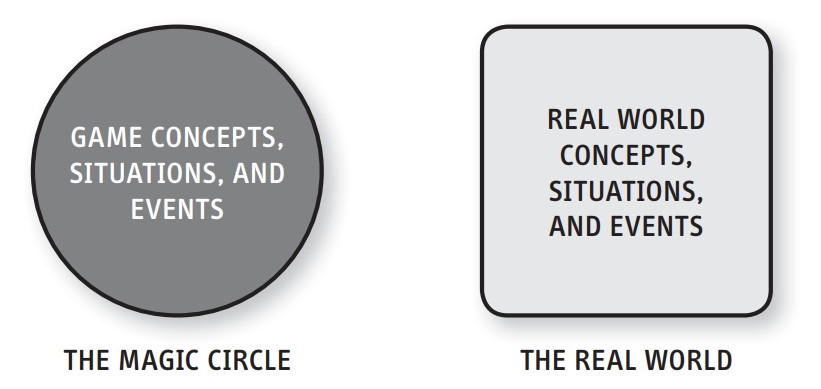
\includegraphics[width=\textwidth]{./Pictures/res/fundamentals/magic-circle}
    \caption{Magic Circle~\cite{10.5555/2544002}}
    \label{fig:magic-circle}
\end{figure}
\\
\\
\textbf{Goals} need to be set in order to correctly design and implement a game.
During the play-through, there always have to be objectives to the user.
Even though a game may seem very goalless, there may be some unseen goals such as acts of creation.
\\
\\
\textbf{Rules} instruct the player through the game and give a boundary or limit to the game.
They are used to describe allowed actions during the gameplay, define progression and - if applicable - give a condition to
end the game.
\\
\\
Generally, the definition of a game is very broad and there are different opinions on the definition, however most of them
do not refer to the games' purpose: it may be purely for entertainment, but can also be for studying, training or attracting interest
for a topic, which is especially the case in the scope of this work.

\subsection{Educational Games}\label{subsec:educational-games}
Most games have a certain factor of education, so called \textit{stealth-education} involved, even though not
specifically intended to be educational.
However, there exist also games with the specified purpose of education, this may include simulations, persuasive games,
games for studying and games that support health and growth.
Educational games are a sub-genre of the \textit{Serious Games}-genre and aim to present or solve real world problems,
while maintaining a factor of entertainment.
Different ways of presentation may be used for educational games~\cite[p.43]{10.5555/2544002}.
While this work mainly aims to attract interest for the topic of aircraft system engineering in a fun and entertaining way, it is still
referred to as an education game in this context, as a definitive, wanted and positive side effect of playing the game is
to introduce the user to basic concepts of system design.
This can be seen as the underlying educational problem and challenge, since the borderline of serious games and games solely
for entertainment purposes is relatively non-restrictive.

\subsection{Game Development Stages}\label{subsec:game-design-stages}
There is no unanimous definition of the game development process, however most approaches and perspectives are similar and the different
stages can be categorized as three main stages~\cite{cg:game-design-stages}:
\begin{enumerate}
    \item Pre-production~\ref{subsubsec:pre-production}
    \item Production~\ref{subsubsec:production}
    \item Post-production~\ref{subsubsec:post-production}
\end{enumerate}
During these stages, different tasks and goals have to be accomplished and reiterated, which will be broken down in detail in the chapters below.
By using the digital educational game life cycle as seen in figure~\ref{fig:deglc} by Aslan and Balci, each of the three stages will be placed in context of
educational games specifically.
\begin{figure}
    \centering
    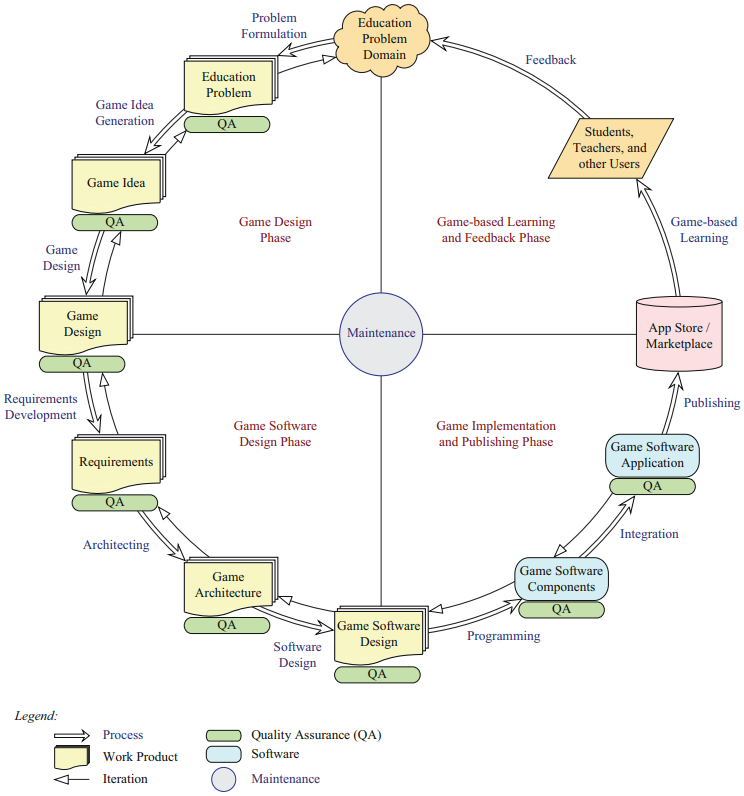
\includegraphics[width=\textwidth]{Pictures/res/fundamentals/deglc}
    \caption{Digital educational game life cycle~\cite{GAMED}}
    \label{fig:deglc}
\end{figure}

\subsubsection{Pre-production}\label{subsubsec:pre-production}
Pre-production is the development stage where only few code is written and the focus lies mostly on defining
problems, laying out ideas and prototyping.
Some important questions have to be answered during the pre-production stage, which are necessary to
head into production and development of the game.
The asked questions focus on the game subject, audience, resources needed and an estimated timespan, as well as
defining the four major elements of a game, as described in section~\ref{subsec:game-definition}.
Sketches and concept art is designed and often, a prototype is developed to show basic layouts of scenes and concepts of game mechanics.
At this stage, when the project team notices flaws or generally bad ideas, game development is either discontinued or the idea and concepts are
reiterated.
The process of pre-production can range in a timespan of a week to multiple months, depending on the size of the project and
the team~\cite{cg:game-design-stages}.
\\
As seen in figure~\ref{fig:deglc}, the first stages in the cycle of educational game development - problem formulation, game idea generation and game design
- represent the idea of a pre-production stage fairly well,
as the main focus is to define the educational problem or subject that has to be solved or taught and why it would be more effective
to do so using a game approach.
Furthermore, requirements to the game and possible approaches to architecture and software design are defined and reiterated.
Note, that even during the next stages, there may be reiterations going back to a previous phase or stage.\ref{GAMED}.
\\
The notable products of the pre-production stage are concepts, ideas, design choices and in the case of educational games an approach to solving and identifying
an existing problem;
and a possible prototype of the idea.

\subsubsection{Production}\label{subsubsec:production}
As production begins, the outlined concept is developed, and code is generated.
It is recommended to follow programming best practices during the coding process to enhance maintainability.
These practices include using well-named variables, classes, and methods in accordance with programming language standards,
as well as incorporating code documentation (e.g., Javadoc), code formatting, and tools for debugging, testing, and logging.
The game framework, engine, and components are programmed to effectively establish the game.
\\
In professional game production, various milestones are set throughout this phase.
After prototyping, the initial milestone is the creation of a playable game that offers a clearer understanding of gameplay
and graphic design, with placeholders replaced by actual graphics.
Subsequently, a fully playable and more insightful project is completed, referred to as a vertical slice.
\\
Finally, during the pre-alpha stage, actual content generation, such as levels, characters, and other elements, is integrated into the game.
During the pre-alpha stage, game features continue to be developed.
However, once the game reaches the alpha stage,
it is considered complete in the sense that it is fully playable from start to finish.
The primary goal at this stage is testing and fixing bugs.
\\
As the game progresses to the beta stage, content creation is finalized, and no new features are introduced.
The focus shifts to optimizing the existing elements rather than implementing changes or adding new components.
\\
The final state of the game, which should also be the end of production stage, is a finished game, which is fully playable and can be
released and used to and by the public~\cite{cg:game-design-stages}.
\\
At the end of the production stage, the framework is clearly laid out and well documented, as well as the game itself is finished for publication~\cite{GAMED}.

\subsubsection{Post-production}\label{subsubsec:post-production}
The post-production stage mainly focuses on maintenance, patches and bug fixes to the finished game, as there are more people playing and therefore more bugs
are found.
Feedback is given to the developers, which may be implemented in future projects.
Usually, this ends the game development process, as there are no new added features (except DLCs - downloadable content, or other add-ons) to the game anymore~\cite{cg:game-design-stages}.
In the case of learning focused or educational games, there may be more iterations of the process, which take the feedback and results of the project into
consideration and develop a new, revised version of the application to create iterations with improved performance, entertainment or educational value~\cite{GAMED,10.5555/2544002}.

\subsection{Game Engines}\label{subsec:game-engines}
Game engines are software frameworks that game developers use to create video games more efficiently.
They provide a set of tools and features that allow developers to create games without needing to build everything from scratch.
Game engines typically provide a range of features, including graphics rendering, physics simulation, audio processing, animation, scripting, and networking.
\\
Game engines come in various forms, from open-source engines that can be freely used and modified by anyone, to commercial engines that require a license fee to use.
Some examples of popular game engines include Unity, Unreal Engine and CryEngine.
\\
Game engines can help reduce the time and cost of game development by providing pre-built components and tools, allowing developers to focus on creating the game's content and gameplay mechanics instead of building the underlying technology.
Additionally, game engines can make it easier to create games that run on multiple platforms, such as desktop computers, mobile devices, and gaming consoles, by providing cross-platform support.
\\
Game engines have become an essential part of the game development process, and have helped democratize game development by making it more accessible to independent developers and small studios.
\\
The above-mentioned game engines use different approaches and concepts, which are pointed out here to give an overview over the generally possible approaches to
designing and developing game engines.
Generally, game engines are developed in high level languages, e.g.~C\#, Java or C++, the reason being object-oriented programming,
which allows general concepts such as inheritance, polymorphism, encapsulation and abstraction to create reusable, maintainable and modular code.
\\
Developing a custom game engine can offer several benefits, such as tailoring functionality and performance for the unique aspects of the project, while
retaining full control and flexibility over new features and the architecture.
Furthermore, a custom game engine reduces or avoids the reliance on third parties regarding support and potential updates, as well as mitigates possible
licensing fees or revenue sharing agreements.

\subsubsection{Unity}\label{subsubsec:entity-component-system}
DOTS (Data-Oriented-Technology Stack) is a framework developed by Unity Technologies for high-performance game development.
It aims to help developers create projects that can efficiently utilize modern hardware and run smoothly on various platforms,
including consoles, PCs, and mobile devices.
DOTS is built on three core pillars: Entity Component System, C\# Job System and Burst Compiler~\ref{dots}.
\\
For the unity engine architecture, a generic entity component system (ECS) design pattern is used, as seen in figure~\ref{fig:ecs-unity}.
The basic idea behind using an ECS is to separate object data and behavior into components, respectively systems.
Each entity is a unique identifier for an object within the game, this can be anything from a button to a sound.
Entities consist of a variety of components, while each entity can have different components based on the needs.
A purely graphical entity which shows an image may only consist of a single graphics component, however another entity may contain
a component for graphics, one for sound and another one that holds collision information.
It is important to note, that components never change an entities' behavior, but only contain data that describes the entity.
Systems are responsible for collecting all relevant entities (i.e.\ entities that contain specific components) and processing them.
An example for a system is a rendering engine, which collects all graphical entities \& components and renders them to the screen by
using the data that is stored within the respective graphics components~\ref{dots}.
\\
Entity-Component-System approaches may also be used paired with other approaches of game design and are generally very broadly customizable and adaptable
to specific needs of the developer.
\\
The C\# Job System is a multithreading framework that enables developers to write safe, high-performance multithreaded code.
It helps to utilize the full power of multicore processors by executing tasks in parallel.
This results in improved performance and responsiveness, especially for CPU-bound tasks like physics simulations, AI calculations, and procedural generation~\ref{dots}.
\\
The Burst Compiler is a math-aware, LLVM-based compiler developed by Unity to optimize C\# code for high-performance execution.
It takes advantage of vectorization, cache optimization, and other low-level optimizations to produce highly efficient native code.
By working together with the C\# Job System, the Burst Compiler helps achieve even greater performance gains~\ref{dots}.
\begin{figure}
    \centering
    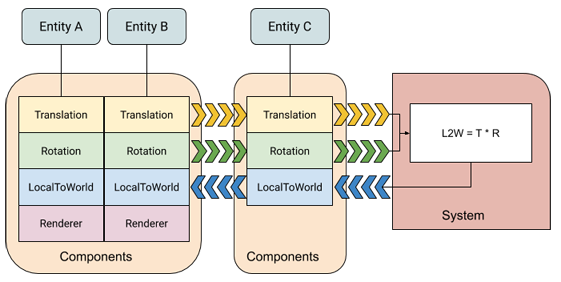
\includegraphics[width=\textwidth]{Pictures/res/fundamentals/ECSBlockDiagram-unity}
    \caption{ECS System used by the Unity Engine \todo{add cite}}
    \label{fig:ecs-unity}
\end{figure}
\subsubsection{Unreal}\label{subsubsec:unreal:-component-based-architecture}
Unreal Engine does not use an Entity Component System (ECS) in the same way Unity does with its Data-Oriented Technology Stack (DOTS) and ECS implementation.
However, Unreal Engine does use a component-based architecture, which shares some similarities with an ECS.
\\
In Unreal Engine, as seen in figure~\ref{fig:unreal-concept}, game objects are represented as Actors, which can have
various components attached to them to define their behavior and appearance.
This approach allows for modularity and reusability of code, which is one of the primary goals of an ECS.
\\
While Unreal Engine's component-based architecture has some similarities with an ECS, it does not follow the strict separation of
data and logic that characterizes an ECS. In an ECS, entities are simple identifiers, components hold only data, and systems
handle the processing of component data.
This separation of concerns allows for better performance and scalability, particularly on modern hardware with multiple cores, due to the possibility
of separating different systems into multiple threads.
\\
Unreal Engine's component-based architecture, though not a pure ECS implementation, provides a powerful
and flexible way to create game objects and manage their behavior.
This is done by a method which constantly updates each component by using their built-in methods, instead of having different systems accessing and changing data within components.
Developers can still achieve good performance and scalability by carefully designing their code and taking
advantage of Unreal Engine's built-in multi-threading and optimization features.
\\
Furthermore, Unreal Engine has a built-in visual scripting system called Blueprints, which allows developers to create game logic without writing code.
This system enables artists, designers, and programmers to collaborate more efficiently and helps those with little programming experience to contribute
to game development.
\begin{figure}
    \centering
    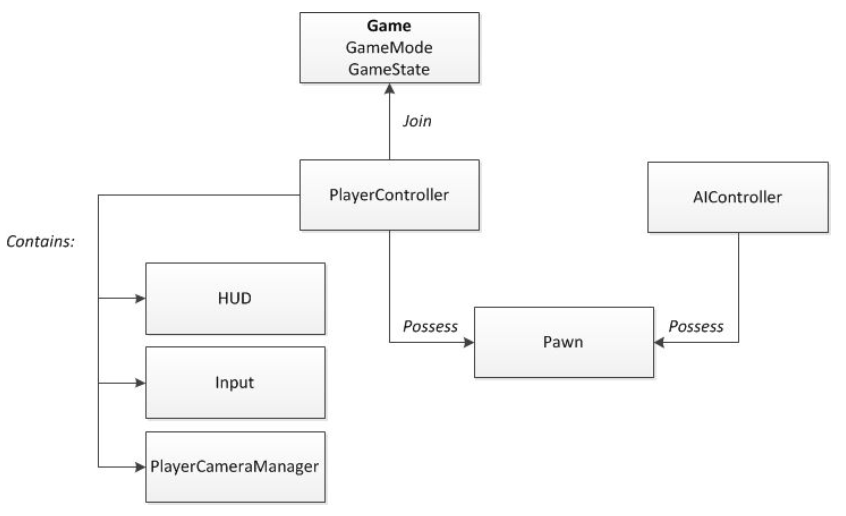
\includegraphics[width=\textwidth]{Pictures/res/fundamentals/unreal-framework}
    \caption{Unreal Architecture~\cite{UNREAL:Framework}}
    \label{fig:unreal-concept}
\end{figure}
\subsubsection{CryEngine}\label{subsubsec:cryengine}
While CryEngine mainly features the same patterns and approaches as Unreal does, one major standout is the very high fidelity graphical rendering
ability.
Particularly real-time rendering and physical based rendering underline this major benefit of using CryEngine, as it enables
creators and designers to create highly realistic environments, for example seen in games like Far Cry, made by Crytek using their own
engine.


\section{Background}\label{sec:background}
In this section, the background to the scope of this work is provided and existing solutions regarding the specified problem and
games with an educational background in general are discussed.
\subsection{Problem}\label{subsec:problem}
The subject of aircraft system design, particularly the concepts of redundancy, can be quite challenging to present and visualize
in an accessible and comprehensive way.
To address this, it is proposed that a gamified simulation is designed, developed, and implemented to have an interactive, engaging way to access the topic of interest.
\\
This interactive game is primarily aimed at young children, as well as learners of all age groups.
It is intended to serve as an educational tool that can be employed during open-house events or as a means of
introducing the subject to individuals with little or no prior knowledge of the topic.
\\
Given that the game is designed to be playable at events such as industry fairs or open-house days,
it should be compatible with external gamepads, including game controllers.
The implementation should involve the use of a game engine to handle the calculations of logic and inputs.
Additionally, a variety of levels should be developed to effectively explain key concepts of aircraft system engineering and
modular integrated avionics regarding safety, such as redundancy, common mode failures, and common cause failures.
\\
The ultimate objective is to provide an enjoyable, interactive visual representation of aircraft system engineering concepts,
while offering direct feedback to facilitate learning.
Players should be able to progress through the levels, experiencing a gradual learning and difficulty curve that sparks interest in the topic
in general and helps grasp and retain the concepts presented.

\subsection{State-of-the-Art}\label{subsec:state-of-the-art}
In the 21st century, e-learning has seen increasing implementation and adoption across various educational levels.
This includes the use of educational games and the integration of game-based learning methods not only in
high schools and universities but also in middle and elementary schools.
One major advantage of using games for educational purposes is that they enable students to experiment,
develop problem-solving skills, and gain a deeper understanding of decision-making processes,
all while receiving immediate visual or auditory feedback~\cite{application-of-education-games-to-enhance-student-learning}.
This is in contrast to traditional learning methods, such as writing essays or submitting homework,
which typically involve delayed feedback~\cite{more-than-just-fun-and-games}.
\\
Furthermore, learning through games can enhance motivation, attention, and retention while offering a flexible learning environment
in terms of both time and location.
However, it is worth noting that students often gravitate towards casual gaming over educational games.
This highlights the need to create engaging and interactive games that are both entertaining and educational to
effectively serve their intended purpose~\cite{WHITTON}.
According to Cheung and Ng~\cite{application-of-education-games-to-enhance-student-learning}, multiple studies in high schools and primary or secondary schools have found that educational
games are more likely to be integrated into the classroom by teachers of higher grades.
Younger learners, who are often more prone to inattention, can particularly benefit from
educational games, as these tools can help improve their attention span and overall learning experience.
\\
This presents an opportunity for the proposed work, which is specifically designed for younger age groups, to make the highly
technical subject of system engineering and redundancy concepts more accessible and engaging through a visual and interactive format
to get the audience interested to possibly learn more in the future and regarding young learners, to maybe start their studies
in this field at a later age.

\subsection{Science Day - University of Stuttgart}\label{subsec:science-day---university-of-stuttgart}
The ``Tag der Wissenschaft'' (Science Day) is an open-door day, where the \textit{University of Stuttgart} can be experienced by everyone.
Exhibits, research environments and results, laboratories and more can be seen, tested and used by everyone, including families, younger children,
high-school students, etc.
It is supposed to show recent research topics and provide insight into the actual work done at the \textit{University of Stuttgart} and to
inform about different studies for interested people who may want to start their studies at the \textit{University of Stuttgart}~\cite{tag-der-wissenschaft}.